\documentclass[tikz,border=8pt]{standalone}
\usepackage{tikz}
\usetikzlibrary{positioning,arrows.meta}

\begin{document}
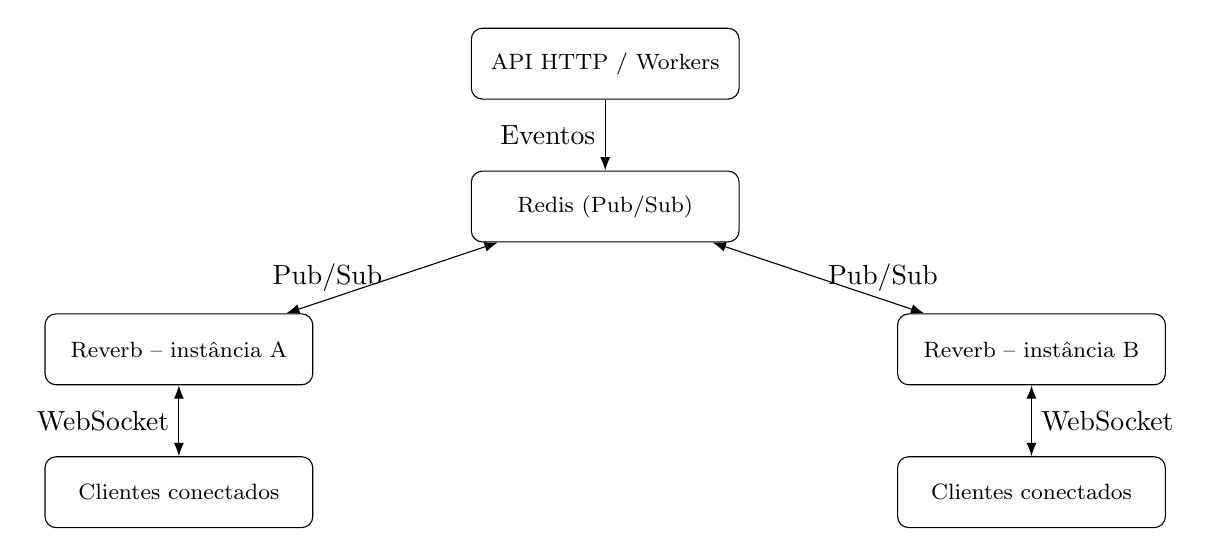
\begin{tikzpicture}[
    node distance=0.9cm and 2.0cm,
    >=Latex,
    box/.style={
        draw,
        rounded corners,
        align=center,
        minimum width=3.4cm,
        minimum height=0.9cm,
        font=\footnotesize
    }
]
    % Camada superior: produtores de eventos
    \node[box] (api) {API HTTP / Workers};

    % Redis central (abaixo da API, mais ou menos no meio)
    \node[box, below=of api] (redis) {Redis (Pub/Sub)};

    % Reverb logo abaixo do Redis
    \node[box, below left=of redis]  (reverbA) {Reverb -- instância A};
    \node[box, below right=of redis] (reverbB) {Reverb -- instância B};

    % Clientes conectados
    \node[box, below=of reverbA] (client1) {Clientes conectados};
    \node[box, below=of reverbB] (client2) {Clientes conectados};

    % Setas de eventos da aplicação para o Redis
    \draw[->] (api) -- node[left]{Eventos} (redis);

    % Pub/Sub entre Redis e Reverb
    \draw[<->] (redis) -- node[left]{Pub/Sub} (reverbA);
    \draw[<->] (redis) -- node[right]{Pub/Sub} (reverbB);

    % WebSockets para os clientes
    \draw[<->] (reverbA) -- node[left]{WebSocket} (client1);
    \draw[<->] (reverbB) -- node[right]{WebSocket} (client2);
\end{tikzpicture}
\end{document}
